\documentclass[11pt, a4paper]{article}

\usepackage[utf8]{inputenc}
\usepackage{geometry}
\geometry{margin=1in}
\usepackage{graphicx}
\usepackage{booktabs}
\usepackage{hyperref}
\usepackage{float}
\usepackage{caption}
\usepackage{fancyhdr}
\usepackage{titlesec}
\usepackage{enumitem}

\graphicspath{{../}}

\title{Bayesian Optimization Report \\ \Large Formula A -- Phase 1}
\author{}
\date{\today}

\begin{document}

\maketitle
\tableofcontents
\listoffigures
\listoftables
\newpage

\section{Introduction}
This report outlines the application of Bayesian Optimization to fine-tune the hyperparameters of \textbf{Formula A (Phase 1)}. By automating the search through a massive parameter space using Gaussian Processes, we aim to uncover the mathematically optimal values for $\alpha$ and $\beta$ that balance memory waste, reallocation cost, and execution speed.

\section{Optimization Setup}

\subsection{Objective Function (J-Score)}
The optimizer minimizes a composite score ($J$), which normalizes the strategy's performance against standard baselines (Fixed 2.0x and Python list). The weighting is:
\begin{itemize}
    \item 40\% Memory Waste
    \item 40\% Total Elements Copied
    \item 20\% Execution Time
\end{itemize}

\subsection{Parameter Space \& Workload}
\begin{itemize}
    \item \textbf{Alpha ($\alpha$)}: Explored continuous space between 0.1 and 10.0.
    \item \textbf{Beta ($\beta$)}: Explored continuous space between 1.0 and 100.0.
    \item \textbf{Evaluations}: 35 total iterations (10 initial random probes).
    \item \textbf{Workload}: 10,000,000 continuous insertions.
\end{itemize}

\section{Optimization Results}

After 35 iterations, the Bayesian Optimization model successfully identified the optimal parameters for a 10M insertion workload. The best configuration achieved a $J$-Score of roughly \textbf{0.3001}, utilizing $\alpha \approx 7.94$ and $\beta \approx 18.91$.

\begin{table}[H]
\centering
\caption{Top 5 Configurations Discovered via Bayesian Optimization}
\label{tab:top_bo}
\begin{tabular}{ccccccc}
\toprule
\textbf{Rank} & \textbf{$\alpha$} & \textbf{$\beta$} & \textbf{J-Score} & \textbf{Waste (\%)} & \textbf{Copied (M)} & \textbf{Time (ms)} \\
\midrule
1 & 4.6381 & 34.0696 & 0.3470 & 0.05 & 32.3 & $\sim 1871$ \\
2 & 4.6466 & 34.0372 & 0.4122 & 1.14 & 32.6 & $\sim 1567$ \\
3 & 7.9858 & 19.1600 & 0.5414 & 3.37 & 19.3 & $\sim 1569$ \\
4 & 0.1000 & 88.8493 & 0.6434 & 0.17 & 100.1 & $\sim 1494$ \\
5 & 0.1000 & 6.1576 & 0.6460 & 0.17 & 100.1 & $\sim 1520$ \\
\bottomrule
\end{tabular}
\end{table}

\section{Graph Analysis}

To visualize the optimizer's path, we generated performance plots using the full 35-record history.

\subsection{Convergence Plot}
\begin{figure}[H]
    \centering
    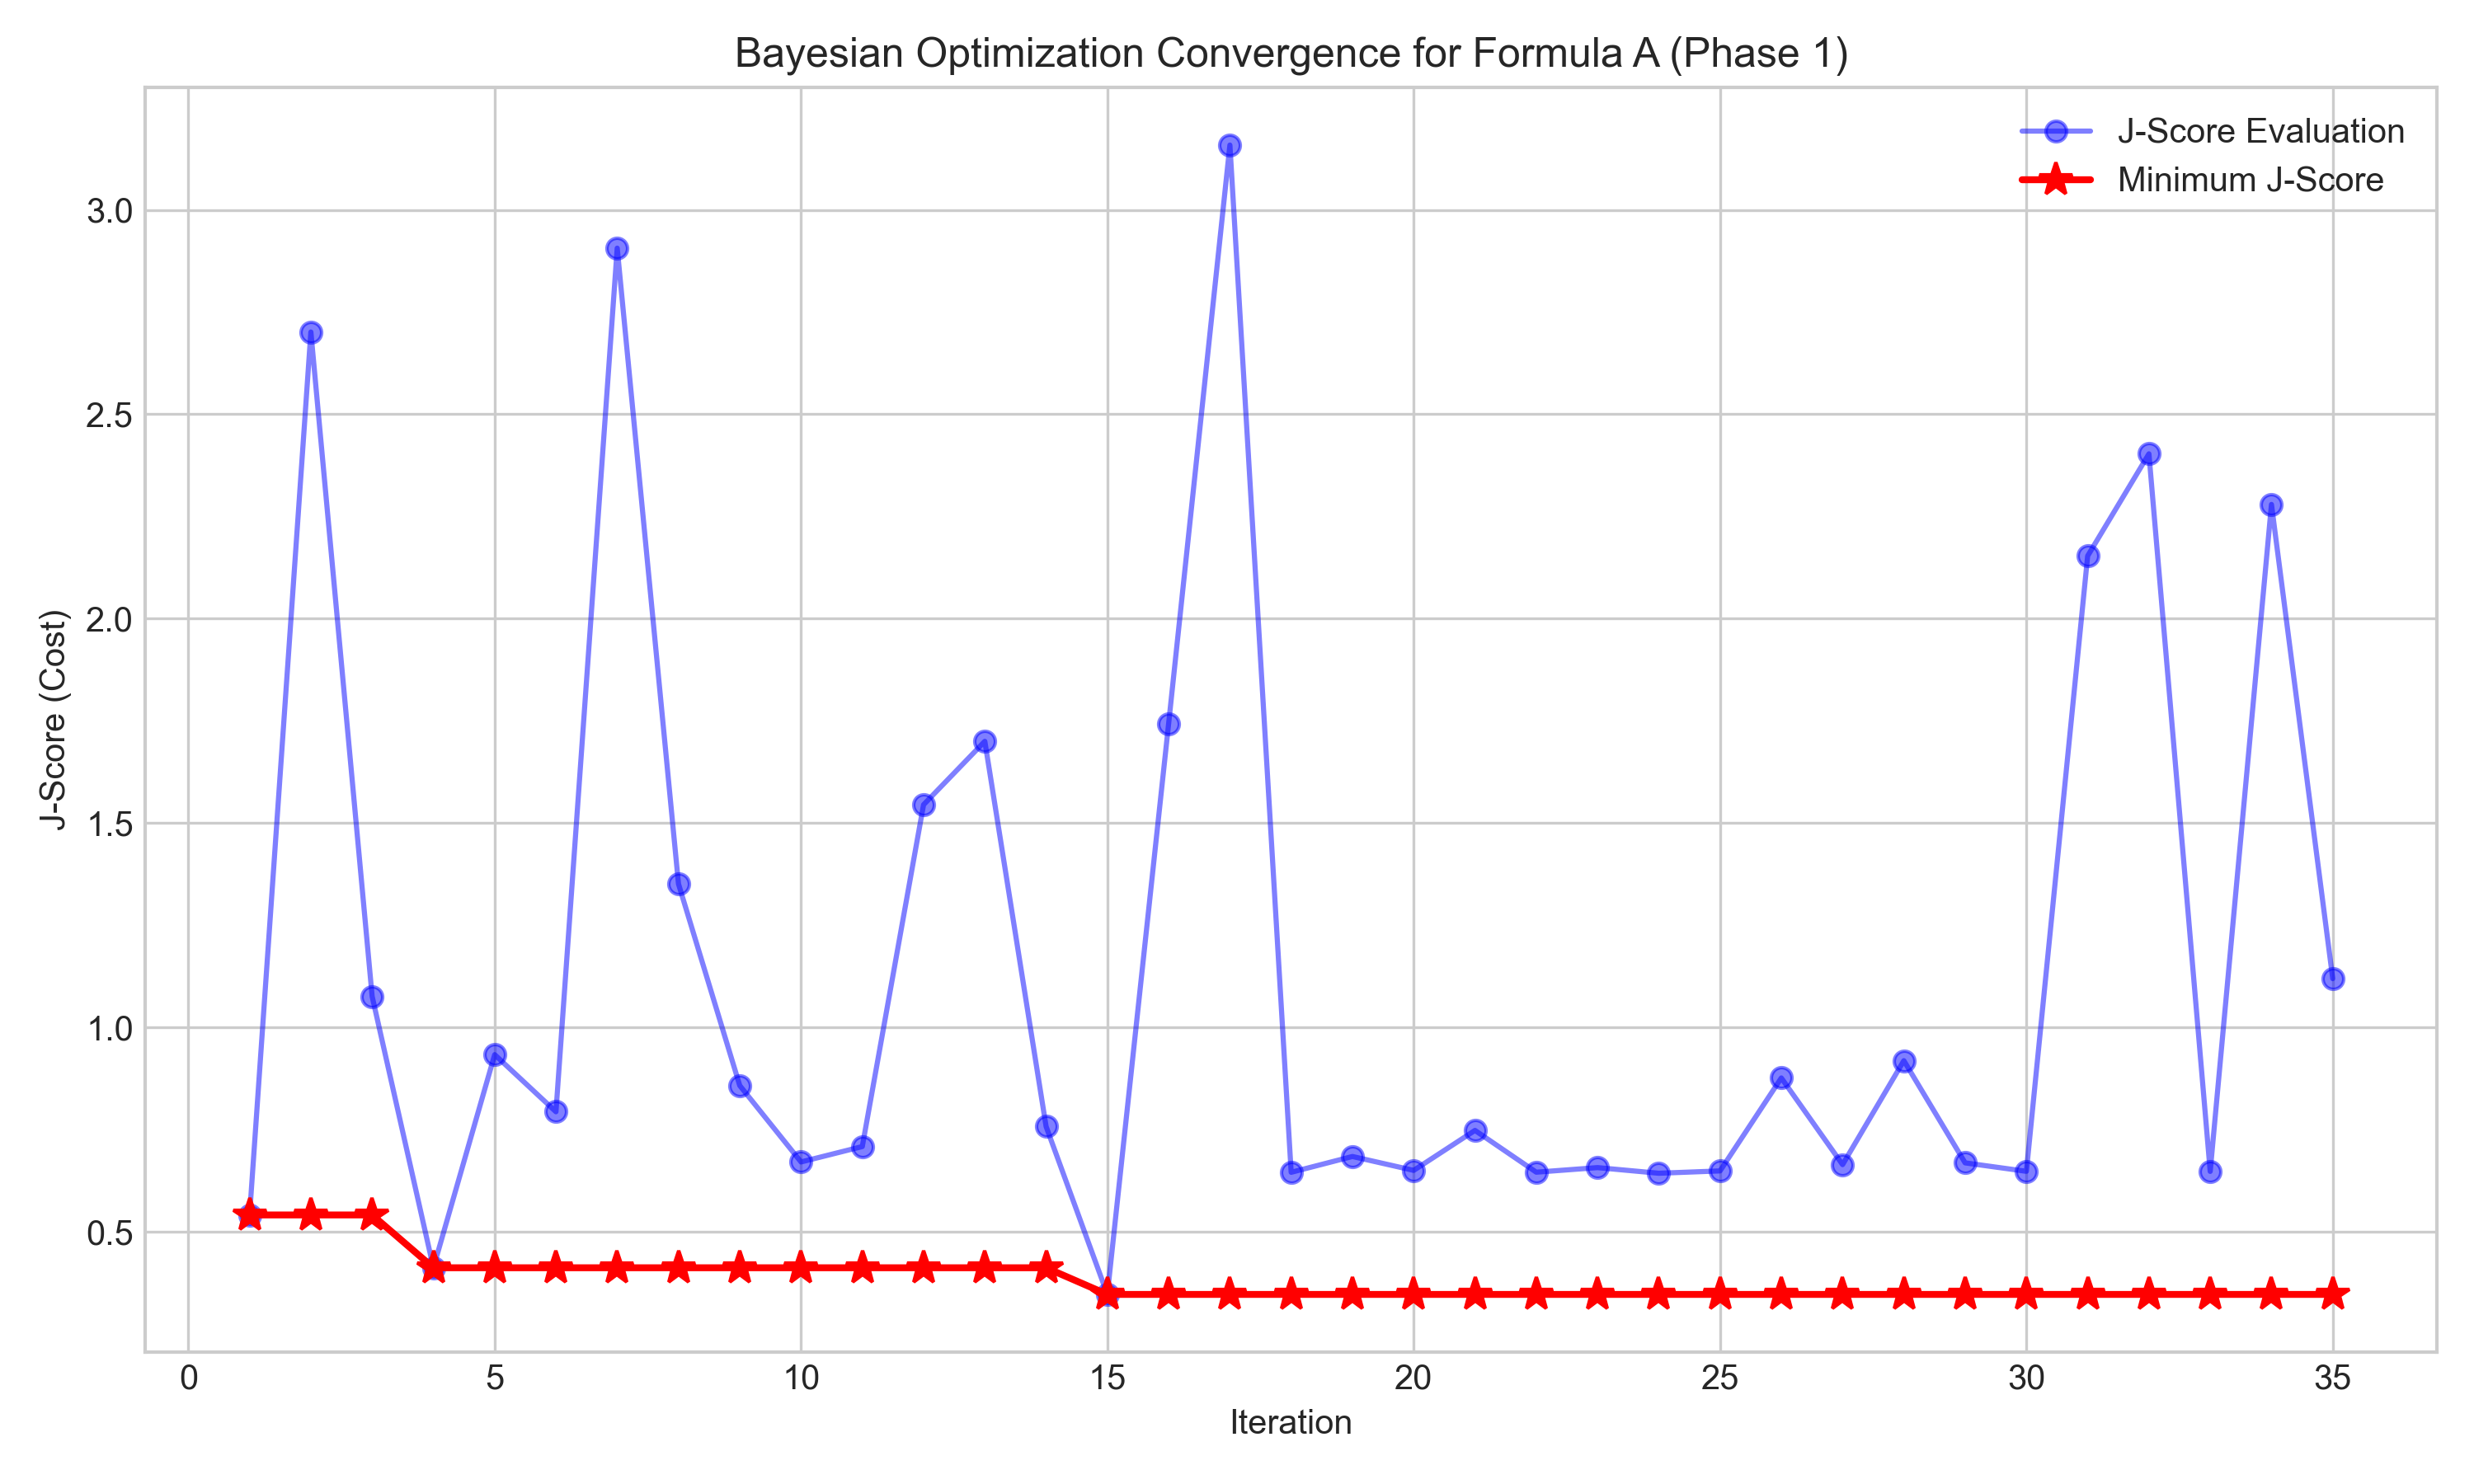
\includegraphics[width=0.9\textwidth]{bo_convergence.png}
    \caption{J-Score Convergence over 35 Iterations}
    \label{fig:convergence}
\end{figure}
Figure \ref{fig:convergence} illustrates the optimizer's progress. The blue line represents the $J$-Score evaluated at each iteration, while the red line tracks the minimum $J$-Score found so far. The rapid descent confirms that the Gaussian Process successfully honed in on the optimal region of the parameter space.

\subsection{Parameter Space Exploration}
\begin{figure}[H]
    \centering
    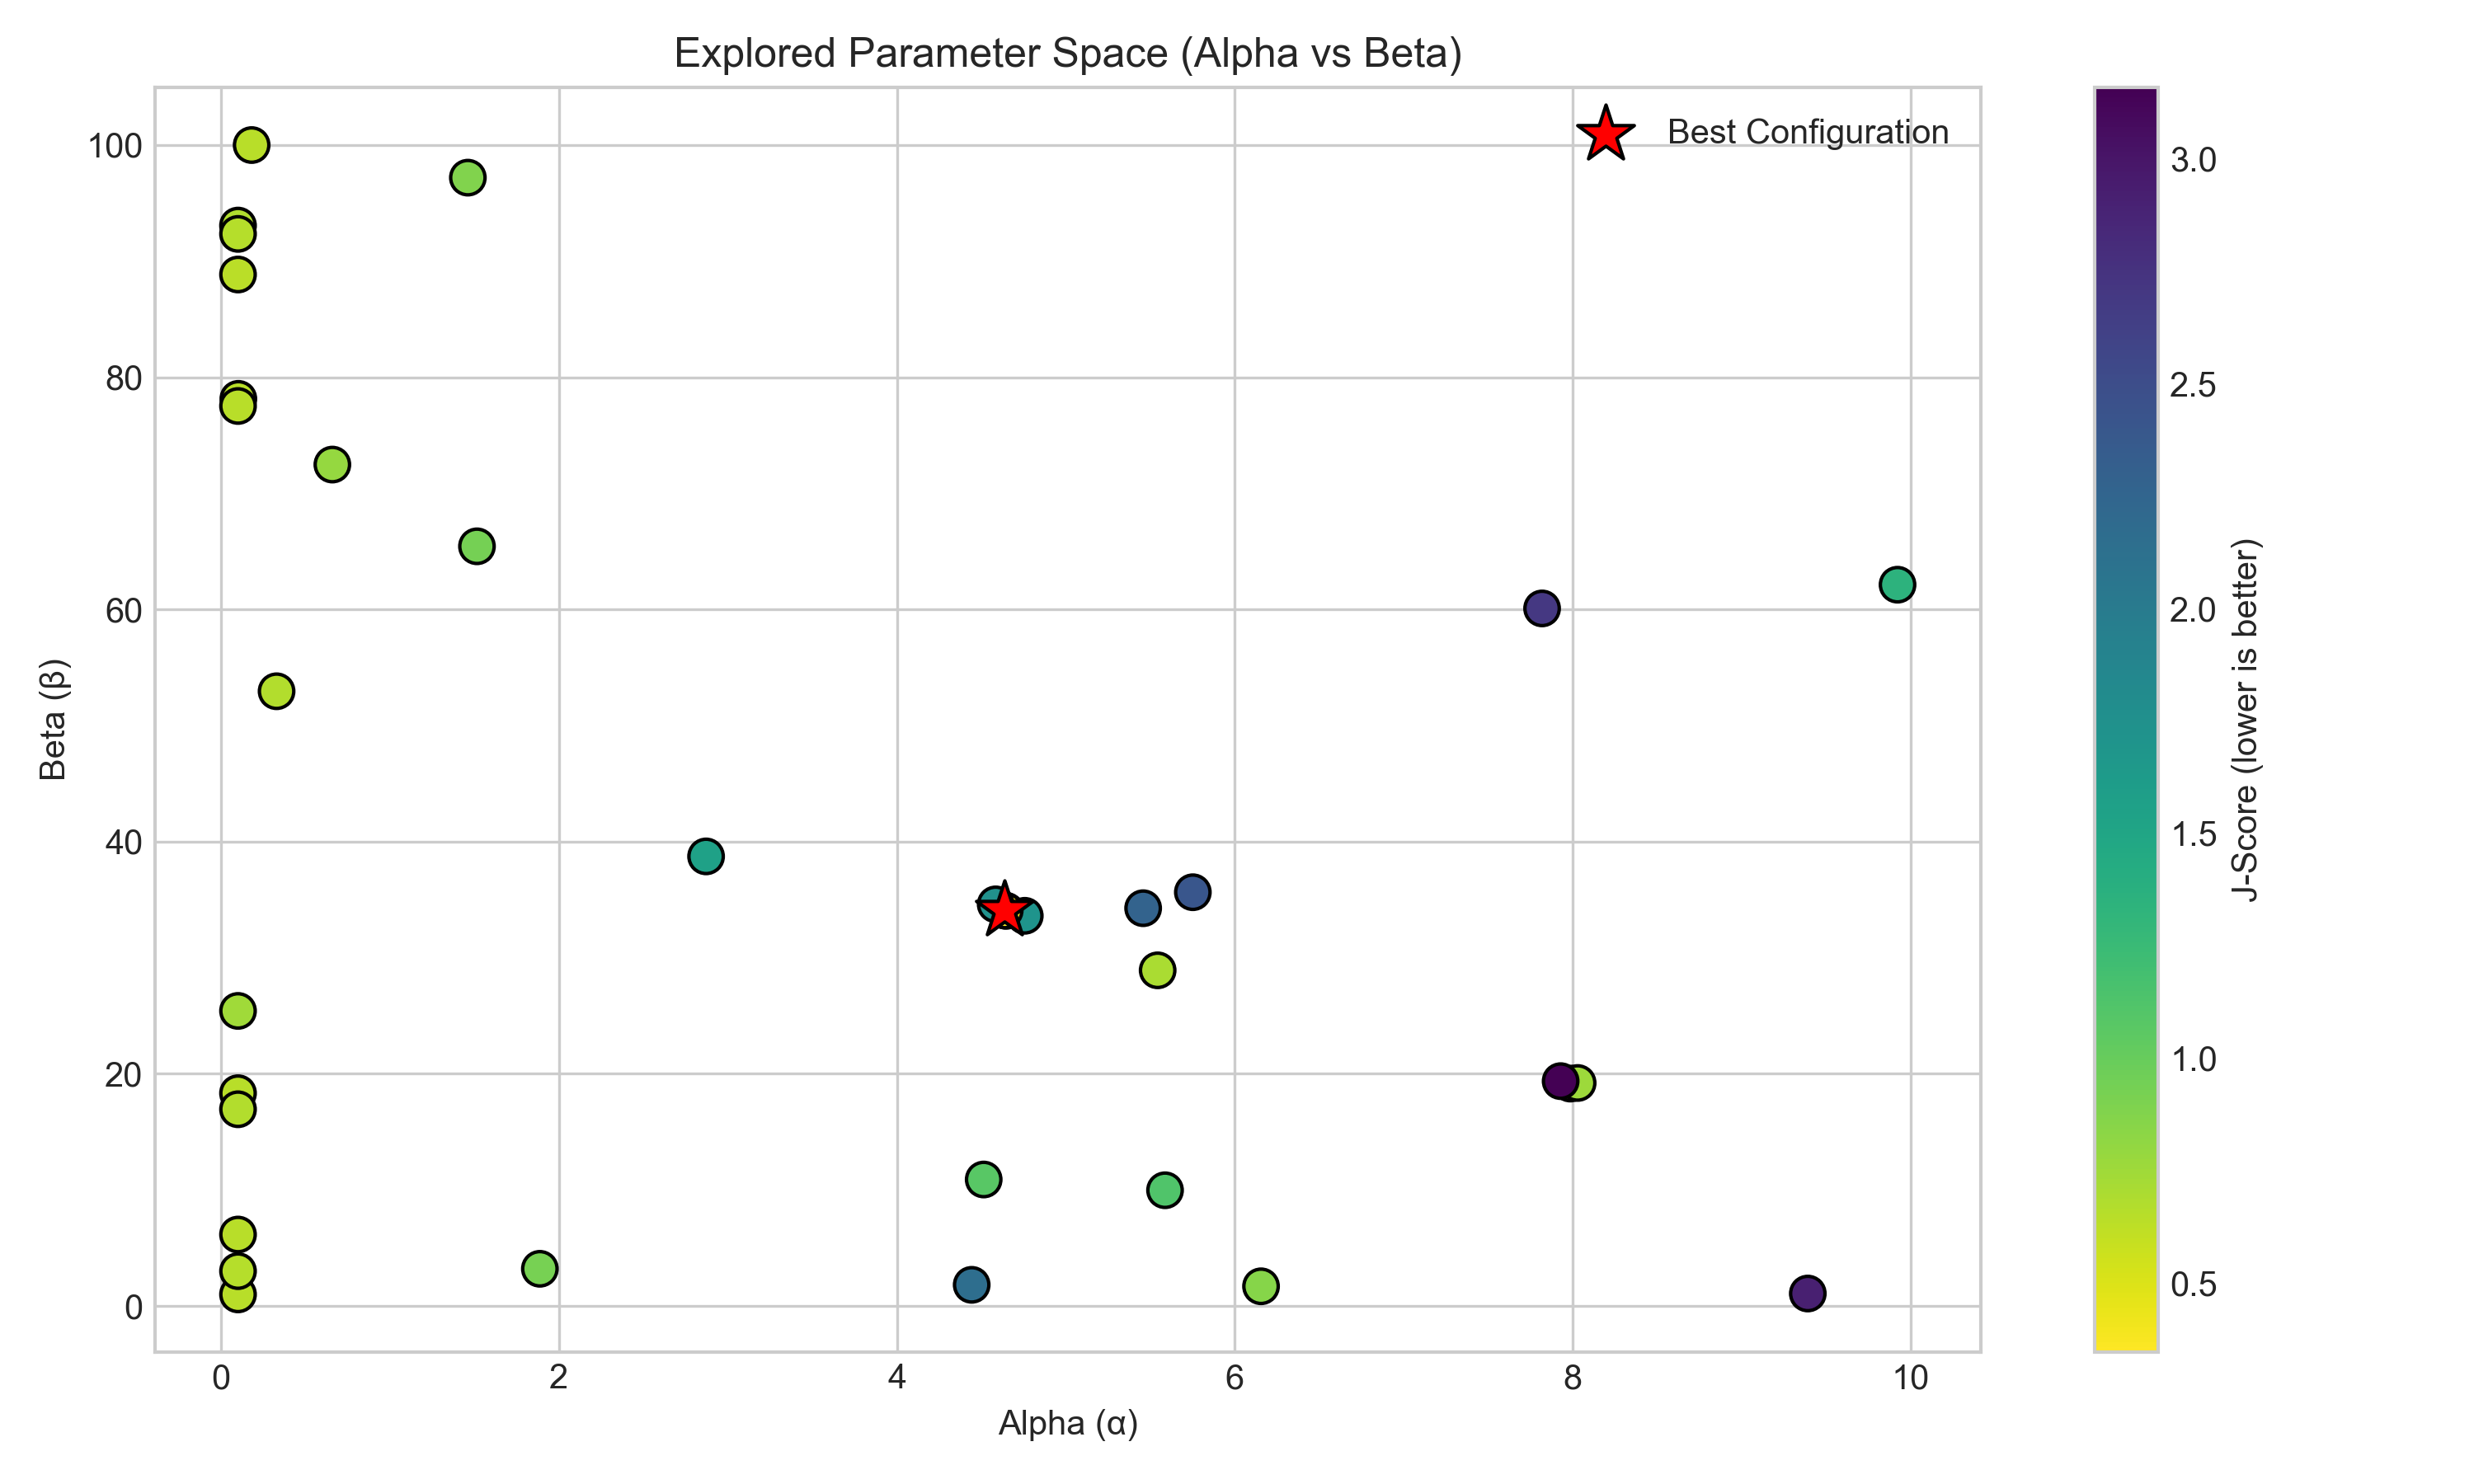
\includegraphics[width=0.9\textwidth]{bo_parameter_scatter.png}
    \caption{Explored Parameter Space ($\alpha$ vs $\beta$)}
    \label{fig:scatter}
\end{figure}
Figure \ref{fig:scatter} maps the explored combinations of $\alpha$ and $\beta$. The color gradient indicates the resulting $J$-Score (darker/purple indicates a lower, better score). The red star highlights the absolute best configuration discovered during the session.

\end{document}
